%%%%% TITLE OF MAIN DOCUMENT %%%%%
%% NUMBER AND TITLE OF SECTION %%


%Some sample text to be displayed above the first subsection

%\subsection{Prinzip}

%Ein Zyklotron besteht aus Zwei hohlen, halbzylindrischen und Duanden an denen eine Spannung mit unterschiedlichem Vorzeichen anliegt, und darüber bzw. darunter liegende Magneten, die ein homogenes Magnetfeld erzeugen. Zudem gibt es einen Einlass und einen Auslass für Teilchen.

%\begin{wrapfigure}{r}{0.4\textwidth} \label{Zyklo}
%
%	\vspace{-10pt}
%	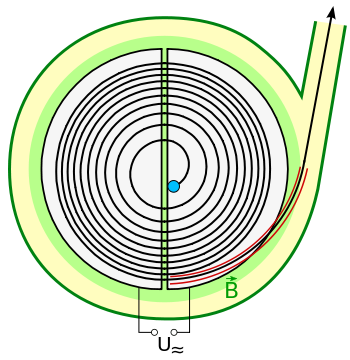
\includegraphics[width=0.35\textwidth]{Zyklotron_Prinzipskizze02.png}
%	\vspace{-13pt}
%	\caption{Prinzipskizze eines Zyklotrons}
%	\vspace{-5pt}	
%	
%\end{wrapfigure}

%\subsubsection{Anwendung}

% Some Formula:

%\begin{equation}
%	x= \frac{y \cdot 13 \pi z}
%			{\cos \alpha}
%\end{equation}

%%%%%%%%%%%%%%%%%%%%%%%
% Eigentlicher Beginn %
%%%%%%%%%%%%%%%%%%%%%%%

Als elektromagnetische Wellen bezeichnet man alle Wellen, bei denen gekoppelten elektrischen und magnetische Felder schwingen. Die Schwingungsverktoren der beiden Felder stehen jeweils senkrecht aufeinander und senkrecht auf dem Vektor der Ausbreitungsrichtung:\footnote{„Onde electromagnetique“ von SuperManu - Self, based on Image:Onde electromagnetique.png. Lizenziert unter CC BY-SA 3.0 über Wikimedia Commons - \url{https://commons.wikimedia.org/wiki/File:Onde_electromagnetique.svg}}

\begin{figure}[h!]
	\center
	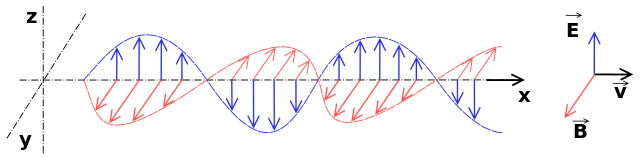
\includegraphics[width=0.8\textwidth]{em_welle}
	\caption{Eine elektromagnetische Welle}
\end{figure}

Im Vakuum bzw. in der Luft bewegen sich alle elektromagnetischen Wellen mit Lichtgeschwindigkeit fort. (Taschenrechner: Konstante 28: $c_0=299.792.458 \frac{m}{s}$)

\subsection{Spektrum}
\hspace{-60pt}
\begin{tabular}[c]{|c|c|c|l|}
	\hline
	Name				&	$f$						& $\lambda$ 	& Kommentar\\
	\hline
	Längstwellen		&	$15-200Hz$				& $10^6-10^7m$ & Strom; Nur Nahfeld\\
	Radiowellen			&	$10^4-10^8Hz$			& $10^0-10^4m$ & \\
	Mikrowellen			&	$10^8-10^{11}Hz$		& $10^{-3}-10^{0}m$ & \\
	Infrarotes Licht	&	$>10^{12}Hz$			& $<10^{-4}m$ & \glqq Wäremestrahlung\grqq \\
	Sichtbares Licht	&	$\approx 10^{15}Hz$		& $400-800nm$ $\approx 10^{-6}m$ & sichtbar\\
	Röntgenstrahlung	&	$10^{16} - 10^{20}Hz$	& $10^{-12}-10^{-8}m$ & Erzeugung: schnelle $e^{-}$ auf Metall \\
	Gammastrahlung		&	$>10^{20}Hz$			& $<10^{-12}m$ & \\
	\hline
\end{tabular}










